\section{Android}

O aplicativo Android é responsável por exibir as informações do servidor web de forma prática e rápida. Ele é compatível versões do sistema superiores ao 4.1 (SDK 16) e possui apenas uma tela. 

Por meio de consultas ao servidor web, o aplicativo lista os registros de ponto. Ele  filtrar os resultados por pessoa, por período (com data de início e data de fim) e também atualizar as informações da consulta que está sendo exibida.

A ~\ref{android_screenshots} mostra as opções disponíveis no aplicativo.

\begin{figure}
\centering
\begin{subfigure}{.5\textwidth}
	\centering
	\caption{Tela Inicial}
	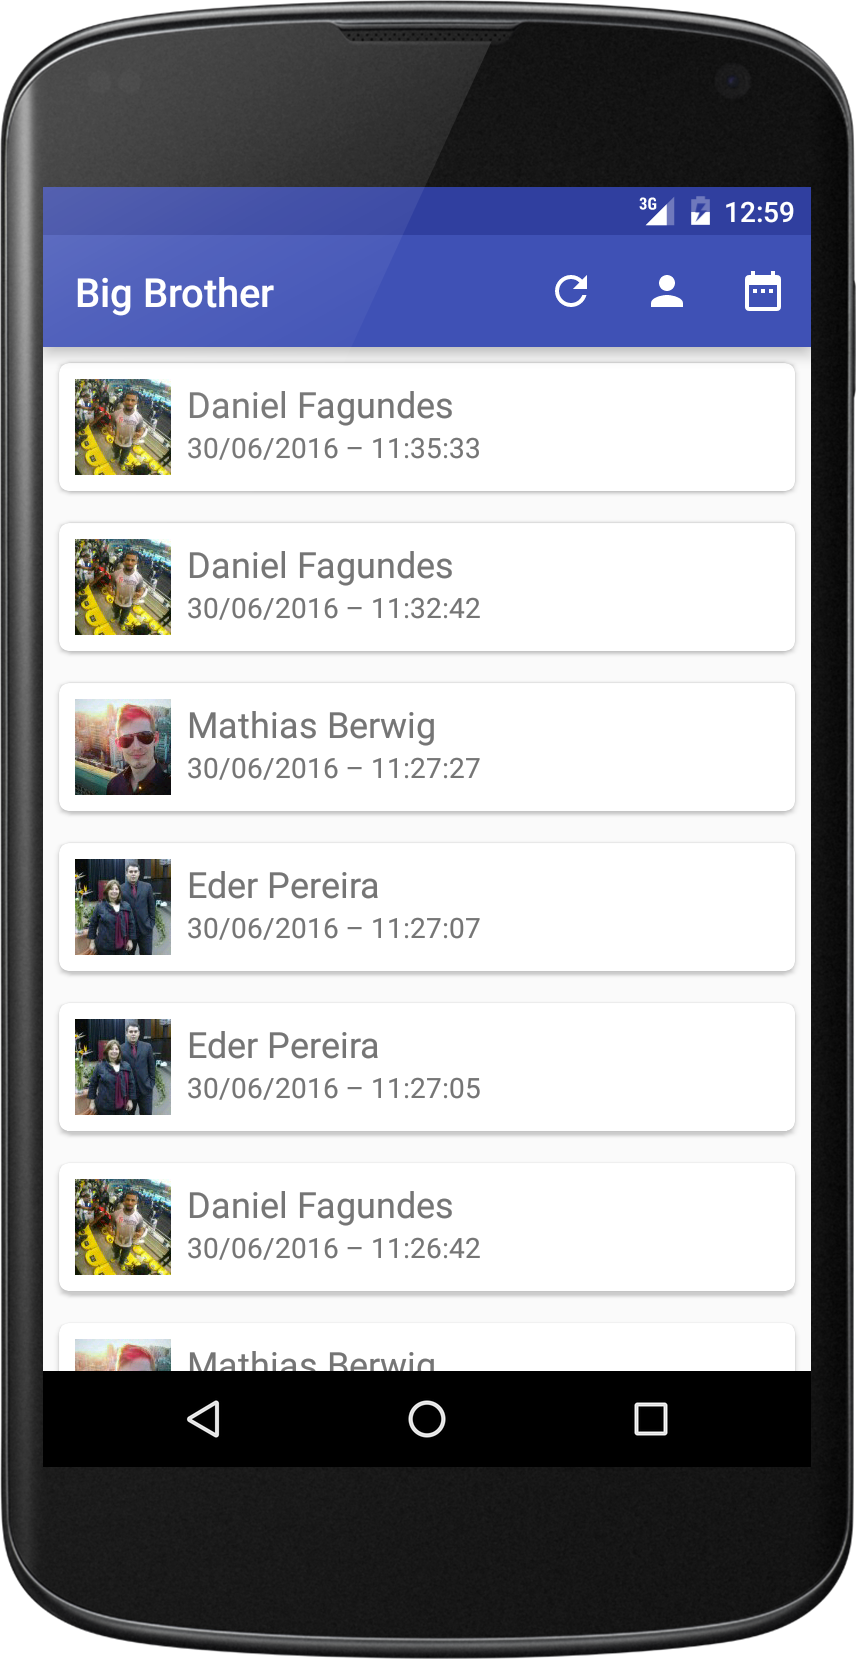
\includegraphics[scale=0.2]{imagens/android_tela_inicial.png}
	\label{android_tela_inicial}
\end{subfigure}%
\begin{subfigure}{.5\textwidth}
	\centering
	\caption{Opção Filtrar Pessoas}
	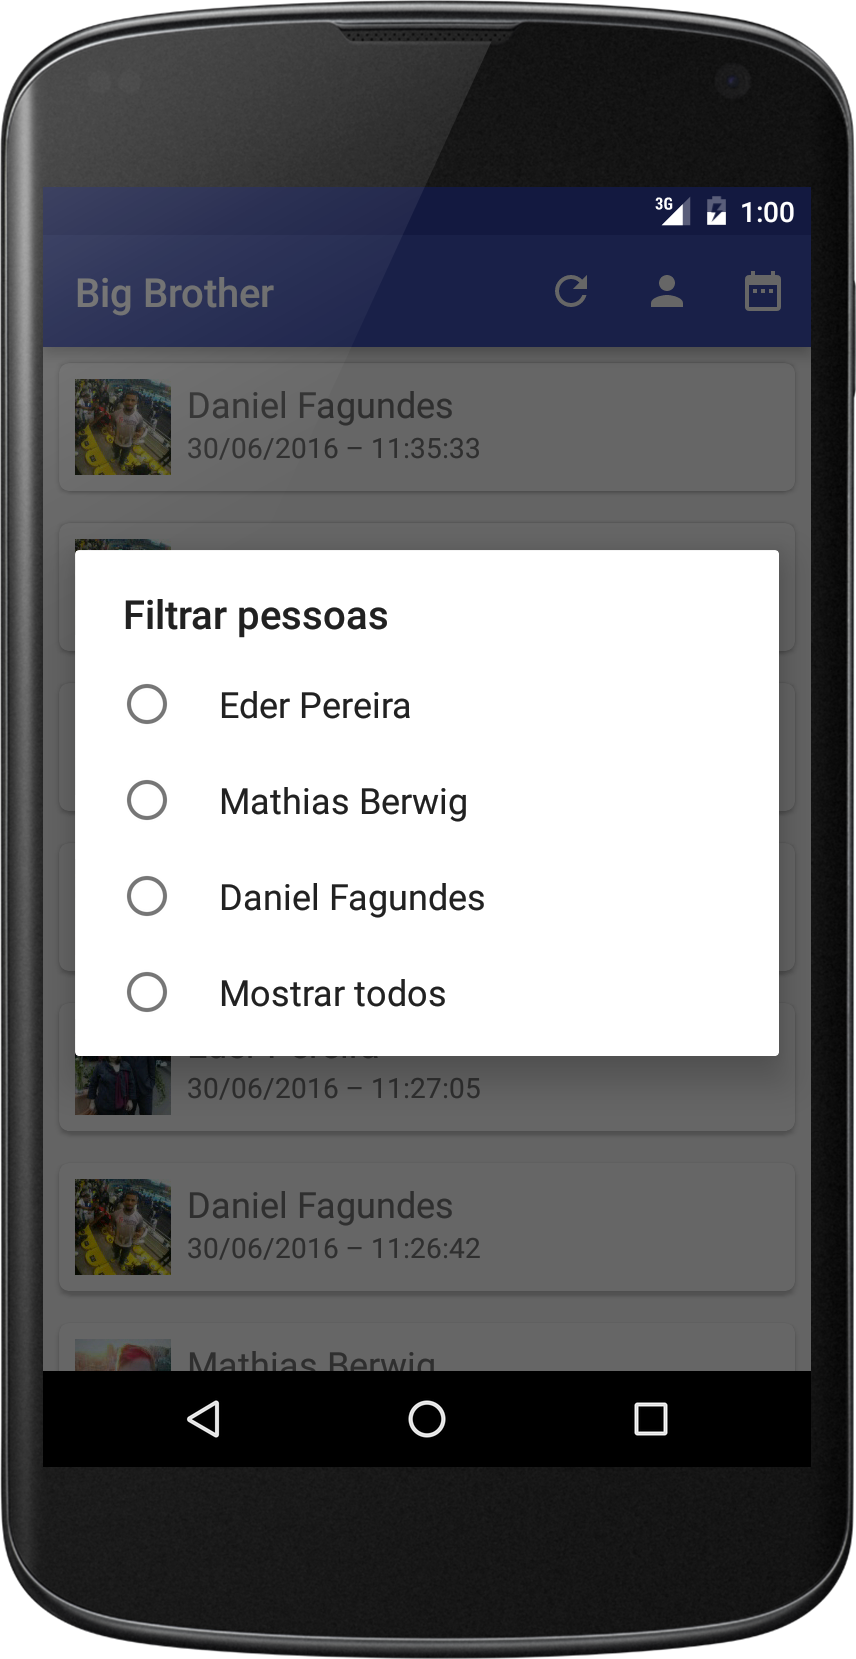
\includegraphics[scale=0.2]{imagens/android_filtrar_pessoas.png}
	\label{android_filtrar_pessoas}
\end{subfigure}
\begin{subfigure}{.5\textwidth}
	\centering
	\caption{Opção Filtrar Datas}
	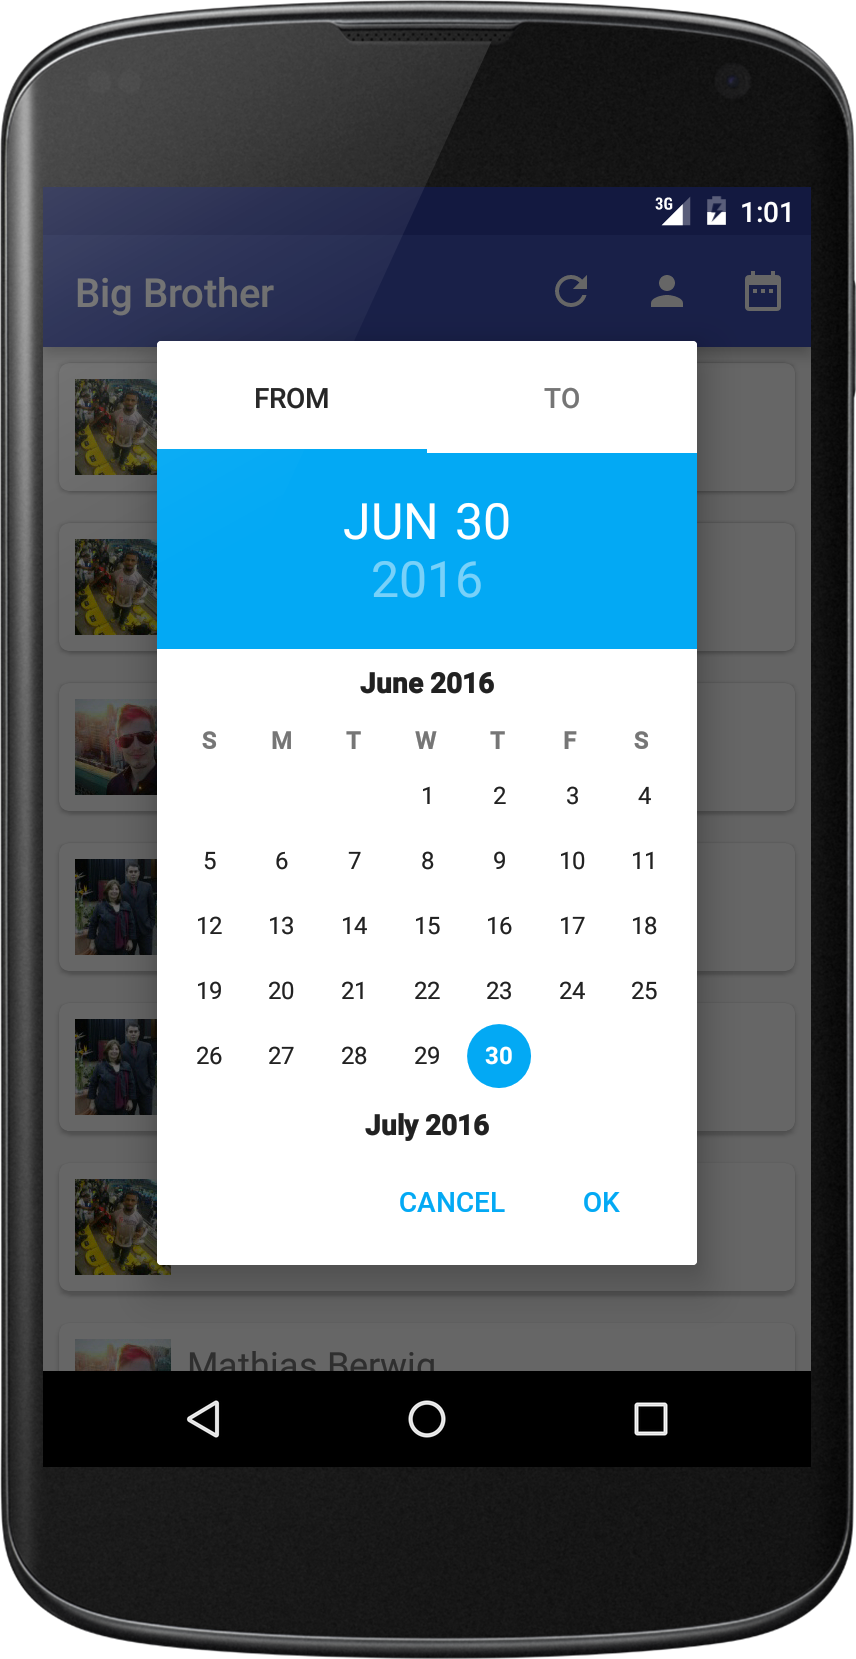
\includegraphics[scale=0.2]{imagens/android_filtrar_data.png}
	\label{android_filtrar_data}
\end{subfigure}
\caption{Capturas de tela do aplicativo.}
\label{android_screenshots}
\end{figure}